%%%%%%%%%%%%%%%%%%%%%%%%%%%%%%%%
\subsection{Contextualiza��o}
% ----------------------------------------------------------------------------
\begin{frame}{Introdu��o}
\begin{itemize}
	\item Intera��es convencionais 
	\begin{itemize}
		\normalsize
		\smallskip
        \item[--] Teclado, \textit{mouse}, \textit{touchscreen}, \textit{joystick}
	\end{itemize}
	\smallskip
\end{itemize}
\vspace{-0.5cm}
\begin{figure}
	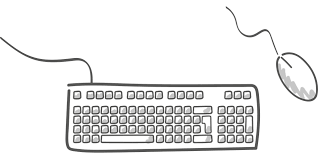
\includegraphics[width=0.3\textwidth]{Figures/mouse1} \quad
	
\includegraphics[width=0.2\textwidth]{Figures/toque}
\end{figure}

\begin{itemize}
	\item Intera��es n�o-convencionais 
	\begin{itemize}
		\normalsize
		\smallskip
		\item[--] Digita��o atrav�s da Fala, Acionador Externo
	\end{itemize}
\end{itemize}

\begin{figure}
	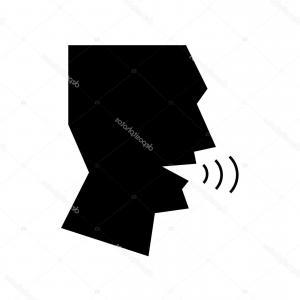
\includegraphics[width=0.2\textwidth]{Figures/talk} \quad
	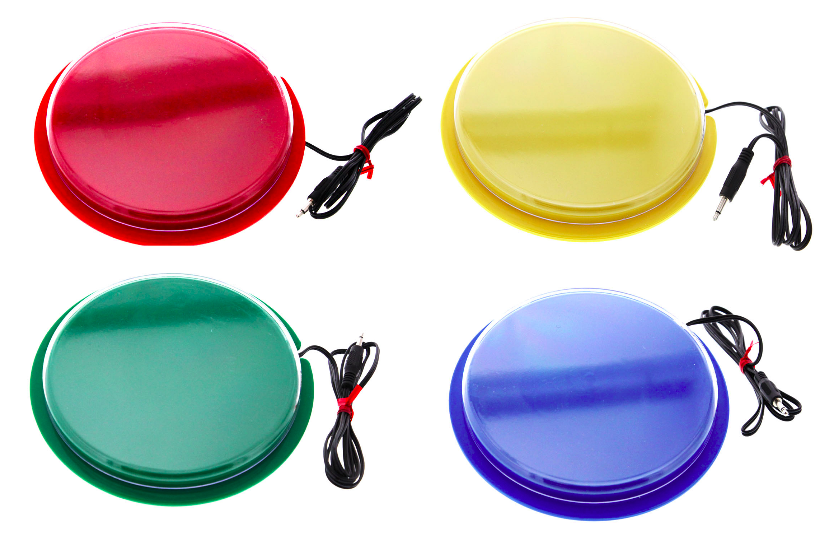
\includegraphics[width=0.2\textwidth]{Figures/at2}
\end{figure}

\end{frame}

% ----------------------------------------------------------------------------
%\begin{frame}{Por que utilizar Acionadores?}
%\begin{itemize}
%	\item Acessibilida
%	\smallskip
%	\item Melhoram a intera��o humano-computador (IHC)
%	\smallskip
%	\item Comodidade e conforto
%\end{itemize}
%\begin{figure}
%	\includegraphics[width=0.48\textwidth]{Figures/jarvis02}
%\end{figure}
%\end{frame}

%%%%%%%%%%%%%%%%%%%%%%%%%%%%%%%%
% \subsection{Motiva��o}
% % ----------------------------------------------------------------------------
% \begin{frame}{Motiva��o}
% \begin{itemize}
% 	\item \textbf{Acessibilidade}: TA para PCD \medskip
% 	\item Tecnologia Assistiva voltada �s pessoas com defici�ncia
% \end{itemize}
% \begin{figure}
% 	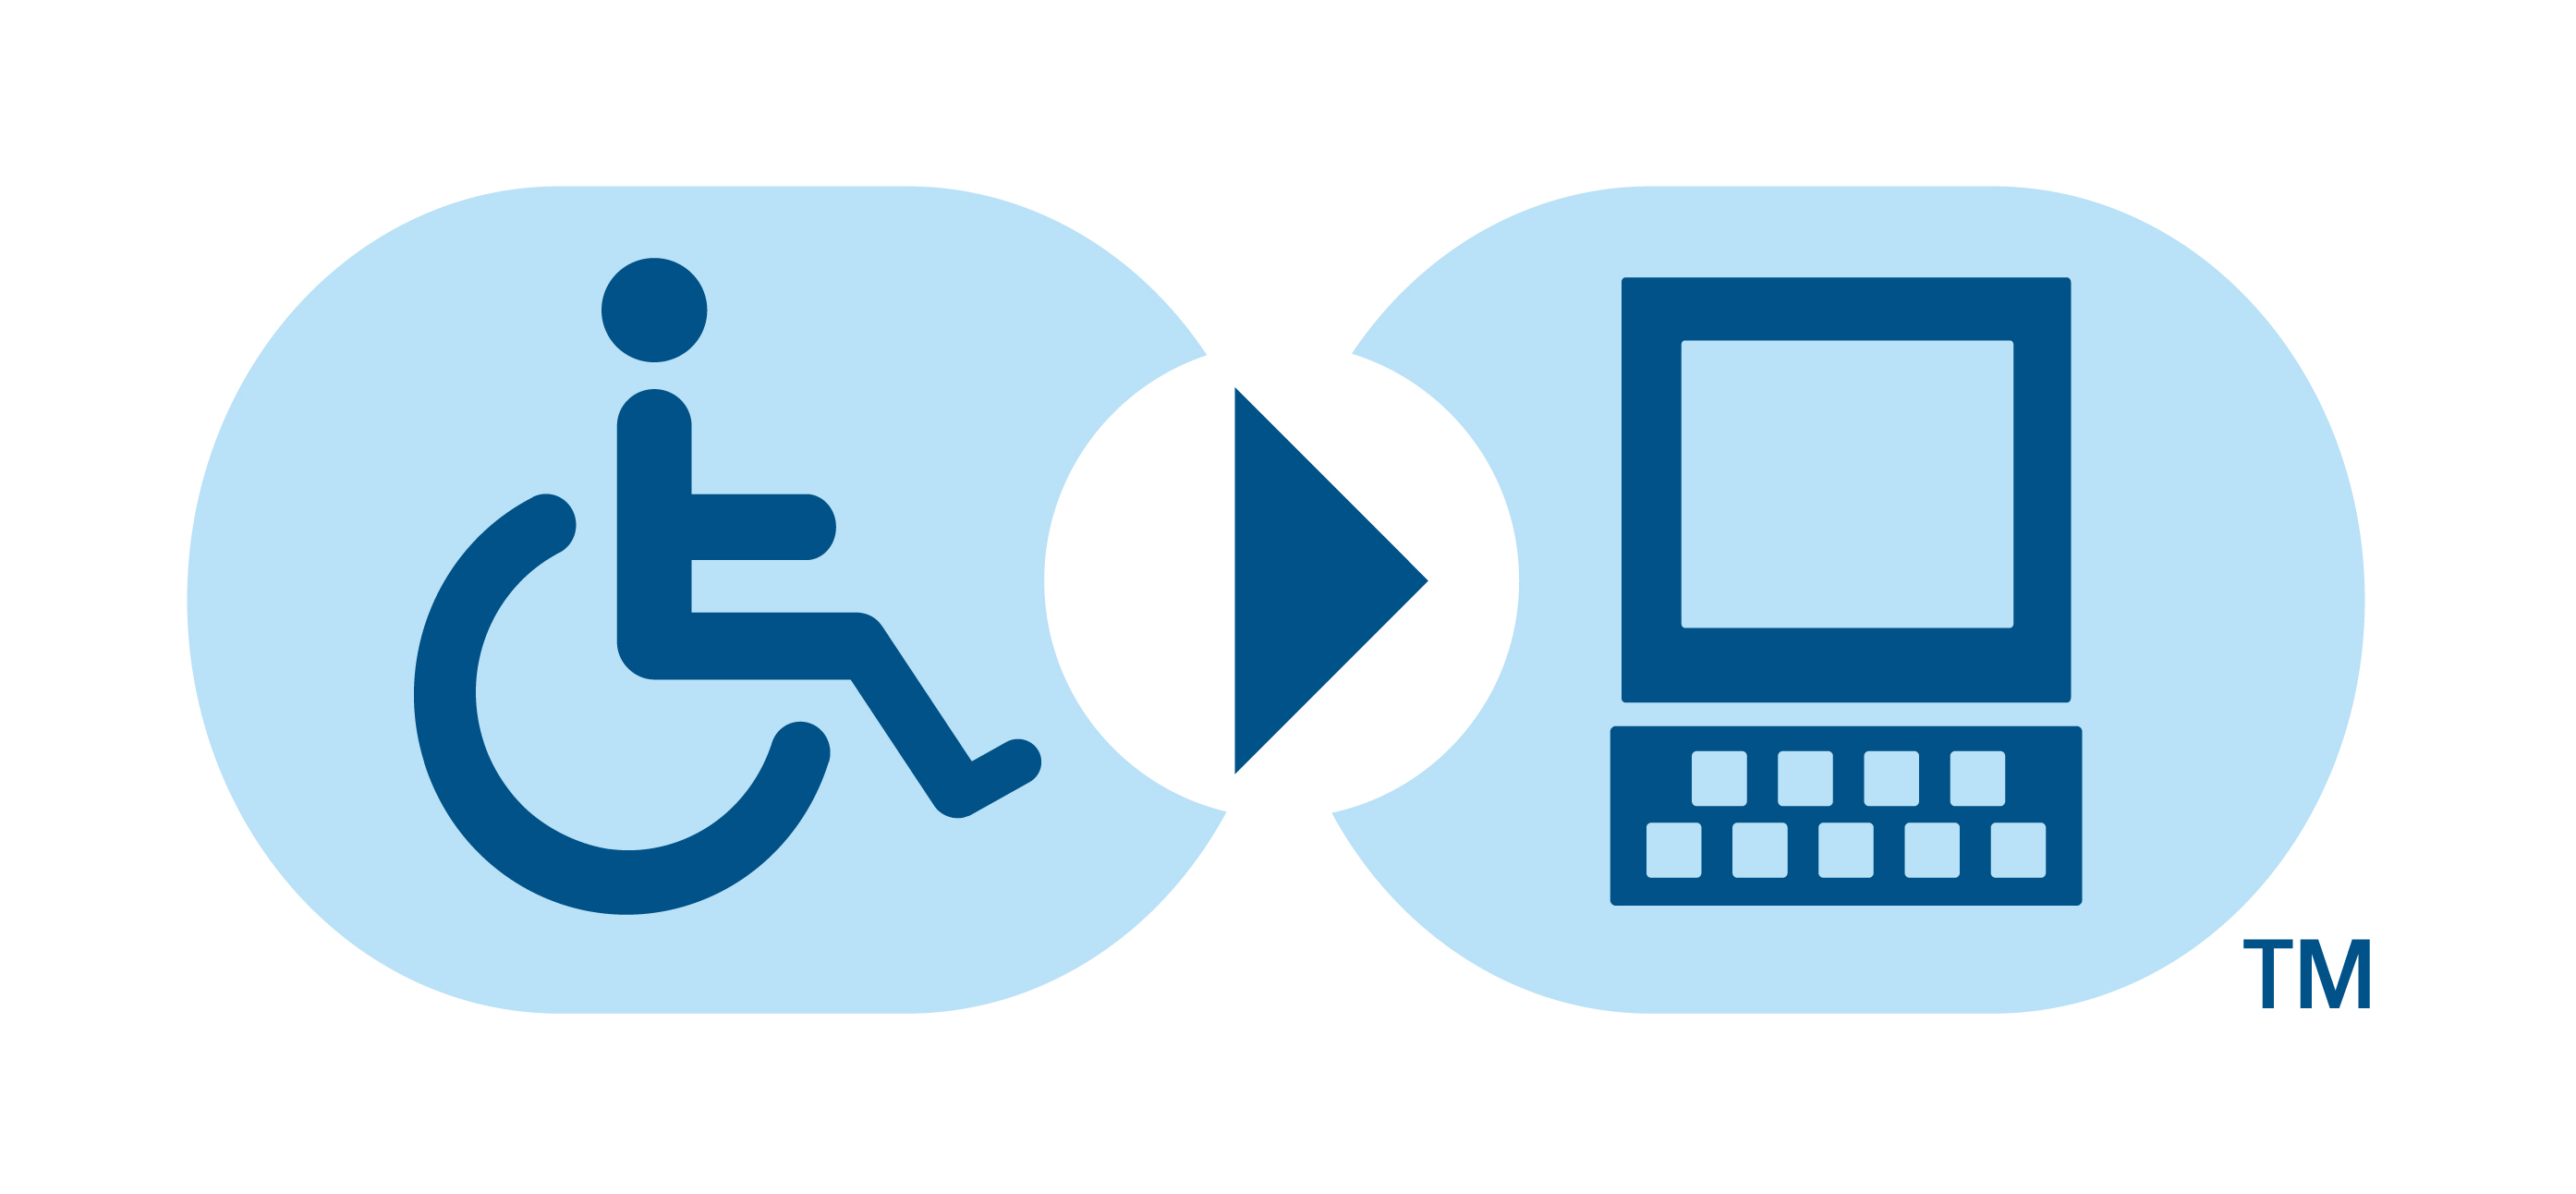
\includegraphics[width=0.80\textwidth]{Figures/access_1}
% \end{figure}
% \end{frame}

% ----------------------------------------------------------------------------
\begin{frame}{Estat�sticas da Popula��o com Defici�ncia}
\begin{itemize}
	\item Mundialmente: 15\% da popula��o $\approx$ 1 bilh�o de
	pessoas~\textcolor{gray}{\small[OMS, 2015]}
	\medskip
	\item No Brasil: 23,9\% dos brasileiros $\approx$ 46 milh�es de
	pessoas~\textcolor{gray}{\small[IBGE, 2010]}
\end{itemize}
\begin{table}
\centering
\caption{Perfil da popula��o brasileira com defici�ncia}
\begin{tabular}{lcr}
	\hline
	\hline
	{\bf Defici�ncia} & {\bf N�mero de Pessoas} & {\bf Porcentagem} \\
	\hline
	{Visual}          & {35.774.392}            & {18,754}     \% \\
	{\bf Motora}      & {\bf 13.265.599}        & {\bf 6,95}   \% \\
	{Auditiva}        & 9.717.318               & 5,094        \% \\
	{Cognitiva}       & 2.611.536               & 1,369        \% \\ 
	\hline
	\hline
\end{tabular}
\end{table}
\end{frame}

\begin{frame}{Problemas}

    \begin{itemize}
    \item Intera��es Convencionais for�am o uso das m�os
    \item Falta de acessibilidade para PCD
    \item Pre�o dos dispositivos existentes
    \end{itemize}

\end{frame}

\subsection{Proposta}
% ----------------------------------------------------------------------------
\begin{frame}{Proposta do Trabalho}
\begin{itemize}
	\item Controlador de mouse baseado na cabe�a do usu�rio
	\begin{itemize}
		\normalsize
		\medskip
		\item[--] M�todo alternativo de clique
		\item[--] Multiplataforma
		% \begin{itemize}
		% 	\normalsize
		% 	\item[$\hookrightarrow$] Linux
		% \end{itemize}
		%\smallskip
		\item[--] Livre: \textit{open-source} e \textit{open-hardware}
		\item[--] De baixo custo
		\smallskip
		\item[--] Com foco em acessibilidade
		\begin{itemize}
			\smallskip
			\normalsize
			\item[$\hookrightarrow$] PCD motora dos membros superiores
			(MMSS) + cognitivo e movimento da cabe�a preservado
            
		\end{itemize}
	\end{itemize}
\end{itemize}
\end{frame}




\subsection{Justificativa}
% ----------------------------------------------------------------------------
\begin{frame}{Justificativa}
\begin{itemize}
\item Por que utilizar o sopro como m�todo de acionamento?
\end{itemize}
\begin{itemize}
	\item No meio acad�mico:
	\smallskip
	\begin{itemize}
		\normalsize
		\item Dificuldade em encontrar trabalhos que utilizam
acionadores como m�todo alternativo de clique
		\smallskip
		\item Apenas um trabalho de acionador externo baseado em
sopro~\textcolor{gray}{\small[B. Aigner, 2016]}
		\smallskip
		\item  Poucos detalhes do desenvolvimento de
		acionadores externos
		\smallskip 
	\end{itemize}
\end{itemize}

\end{frame}


%\begin{frame}{Justificativa}
%%
%\begin{itemize}
%	\item No mercado:
%	\smallskip
%%\begin{minipage}{0.65\textwidth}
%\begin{itemize}
%	\item[]
%\begin{itemize}
%	\normalsize
%	\item  Comunica��o direta atrav�s da interface de �udio para realizar o clique
%	\smallskip
%	\item  Acionadores externos de alto custo e propriet�rios
%\end{itemize}
%\end{itemize}
%\end{itemize}
%%\end{minipage}
%\begin{figure}
%	\centering
%	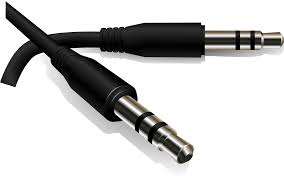
\includegraphics[width=0.3\textwidth]{Figures/ts1}\\
%	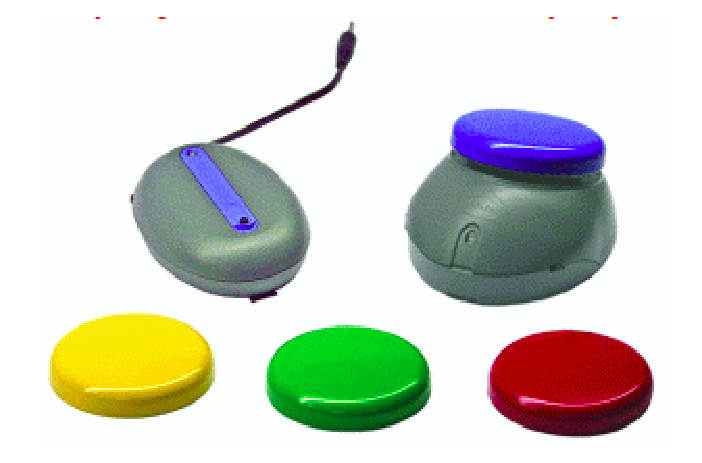
\includegraphics[width=0.3\textwidth]{Figures/at_switch_wireless} \quad 
%	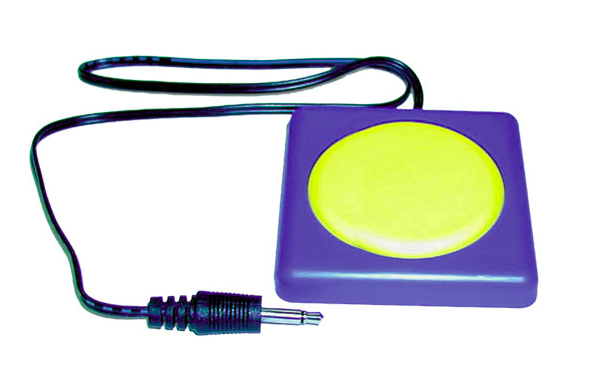
\includegraphics[width=0.3\textwidth]{Figures/at1} 
%\end{figure}
%\end{frame}
%%% EOF %%%

